\section{Schwächen der Textursynthese und deren Verbesserungsmöglichkeiten}

Bisherige Ansätze demonstrieren ihre Algorithmen nur für Beispielmustern mit geringen Auflösungen bis zu $128^2$ Pixeln \cite{SelfTuning}.
Für diese Auflösungen funktionieren die vorgestellten Ansätze gut, denn die entsprechenden Beispielmuster enthalten auf Grund ihrer geringen Größe oftmals nur kleine Details, die sich leicht vervielfachen lassen, ohne dabei unnatürlich auszusehen.
Höher aufgelöste Beispielmuster leiden dagegen an der \glqq Markov-Random-Field\grqq -Eigenschaft.
Es werden stets nur kleine lokale Ausschnitte eines Beispielmusters betrachtet, wodurch die globale Ähnlichkeit zu dem benutzten Muster völlig außer Acht gelassen wird.
Folglich werden Texturen aus hochauflösenden Beispielmustern synthetisiert, die den Erwartungen qualitativ hochwertigen Texturen nur selten gerecht werden.

In diesem Kapitel wird eine Textursynthese beschrieben, die sich der Texturoptimierung annimmt und sie mit mehreren Verbesserungen ausstattet, um die bisherigen Probleme der Textursynthese zu überwinden.
Dazu zählen insbesondere das Erhalten von großflächigen Strukturen aus dem Beispielmuster, das Vermeiden von auffälligen Wiederholungen in der synthetisierten Textur und das Erkennen und Bewahren von Regelmäßigkeiten.
Das Verfahren greift dabei Schlüsselideen vorangegangener Verbesserungsmöglichkeiten auf und modifiziert sie in so fern, sodass die Texturoptimierung weiterhin völlig autonom arbeiten kann und keine individuellen, benutzerdefinierten Anpassungen für unterschiedliche Beispielmuster von Nöten sind.

\subsection{Großflächige Strukturen}

Texturen bzw. Beispielmuster enthalten oft Details verschiedener Größen.
So enthält eine Steintextur winzige Details in ihrer Oberfläche, aber wohlmöglich auch größere Strukturen wie etwa Risse oder Kanten.
Diese Strukturen mit großer Ausdehnung werden in der bisherigen Synthese garnicht erst berücksichtigt.

Ein möglicher Ansatz dieses Problem zu lösen ist der Einsatz eines \emph{\glqq Guidance-Channels\grqq} \ \cite{SelfTuning}.
Dieser \glqq Guidance-Channel\grqq \ erweitert das Beispielmuster um einen zusätzlichen Kanal, in welchem nicht-lokale Informationen über großflächige Strukturen des Beispielmusters gespeichert werden.
\cite{Guidance} zeigt, dass diese Methode besonders gut funktioniert, wenn in ihm die Distanz jedes Pixels zu dem an ihm nächstgelegenen Merkmal (z.B. eine Kontur)  gespeichert wird.
Dieser \glqq Guidance-Channel\grqq \ soll im Gegensatz zu bisherigen Verfahren völlig automatisiert berechnet werden und nicht explizit durch den Benutzer übergeben werden müssen \cite{SelfTuning}.

\begin{figure}
	\centering
	\begin{subfigure}{0.3\textwidth}
		\centering
		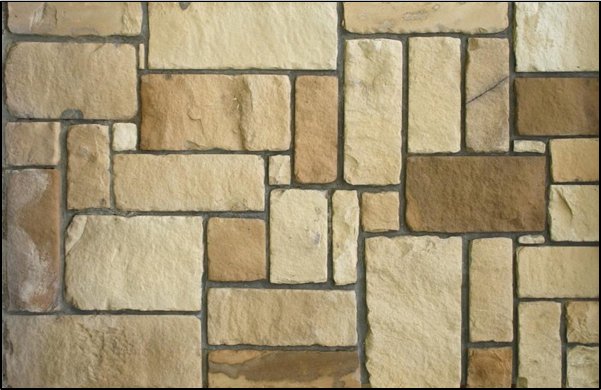
\includegraphics[width=0.8\textwidth]{images/guidance-channel-1}
		\caption{Beispielmuster}
	\end{subfigure}
	\hfill
	\begin{subfigure}{0.3\textwidth}
		\centering
		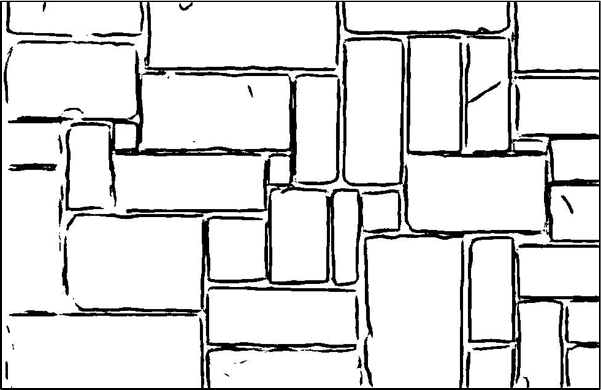
\includegraphics[width=0.8\textwidth]{images/guidance-channel-2}
		\caption{Kantenbild}
	\end{subfigure}
	\hfill
	\begin{subfigure}{0.3\textwidth}
		\centering
		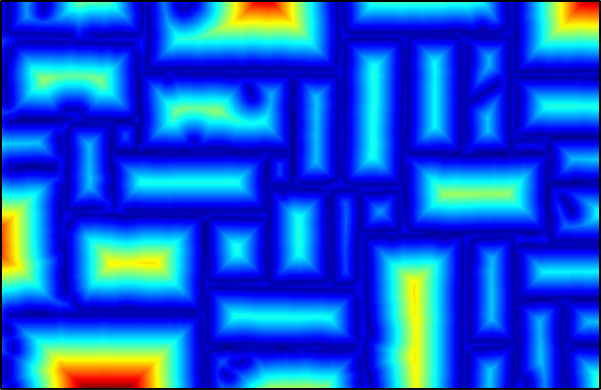
\includegraphics[width=0.8\textwidth]{images/guidance-channel-3}
		\caption{\glqq Guidance-Channel\grqq}
	\end{subfigure}
	
	\caption{Erstellung eines \glqq Guidance-Channels\grqq}
	\label{guidance-channel}
\end{figure}

Die Erstellung eines \glqq Guidance-Channels\grqq \ umfasst mehrere Schritte, die in Abbildung \ref{guidance-channel} illustriert sind.

\subsection{Auffällige Wiederholungen}

\subsection{Regelmäßigkeiten}